\chapter{Finite State Machine (Endlicher Automat)}
Die Finite State Machine ist ein Modell eines Verhaltens. Es ist ein graphischer Entwurf, der flexibel Erweiterbar ist, sowie ein Programmierkonzept.

\textbf{Beispiel Ampel} \\
\begin{enumerate}
	\item Entwurf eines Zustanddiagrammes mit Übergang
	\item Zustand durchnummerieren (wird global gespeichert)
	\item Übergänge sind \texttt{if}-Bedingungen (Ausnahme: sofortige Aktionen)
	\item Zustände sind Methoden: Zeitsensible Übergänge benötigen 2 Zustände (starten und warten)
\end{enumerate}
Ampel: 3s rot, 5s grün
\begin{figure}[H]
	\centering
	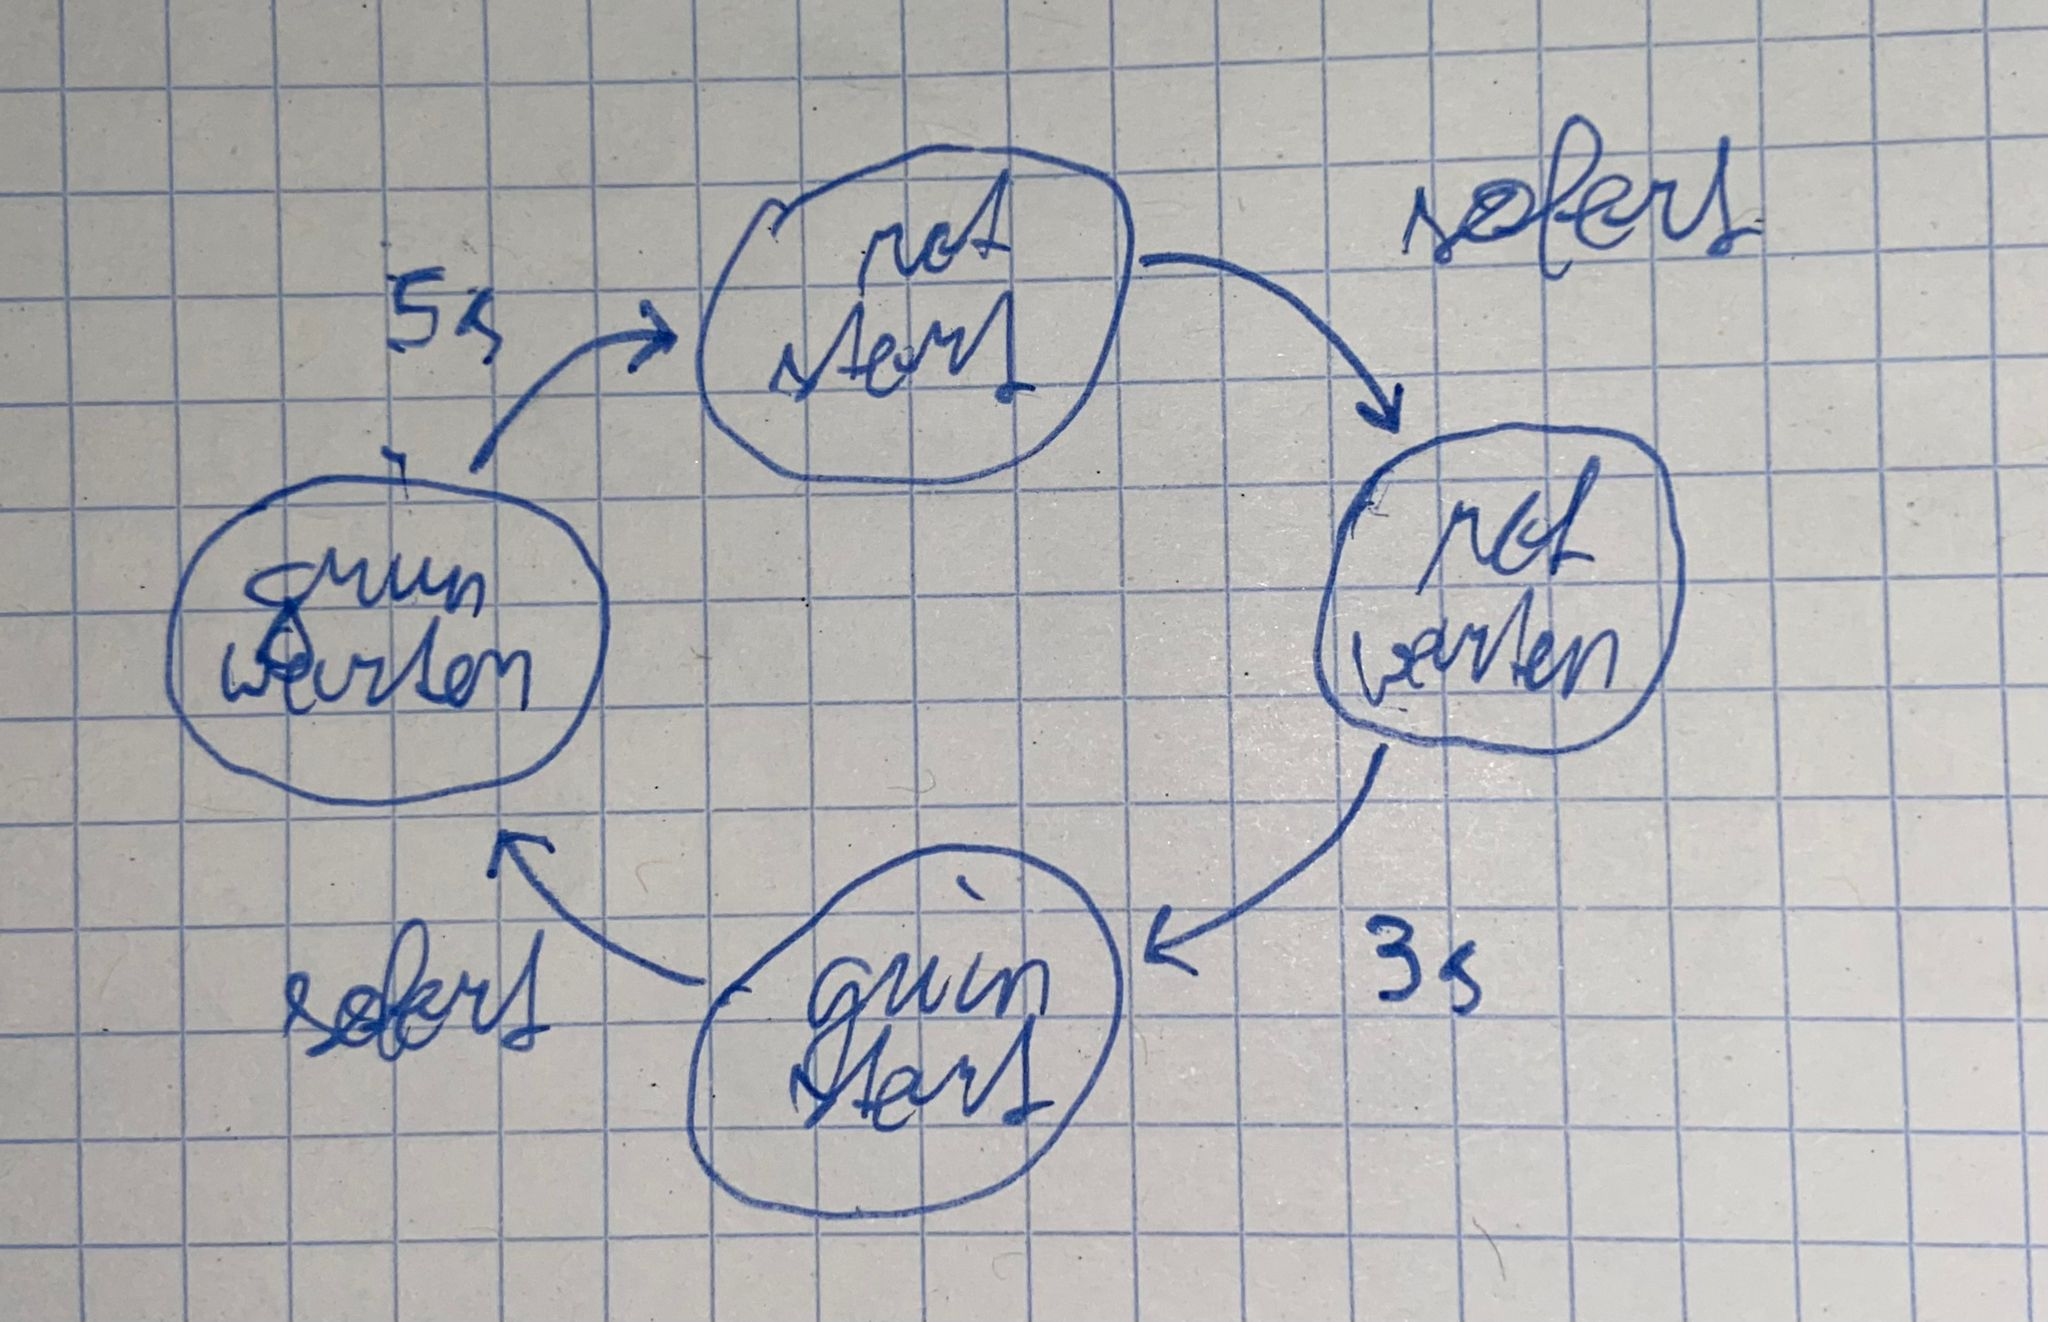
\includegraphics[width=0.8\linewidth]{figures/ampel.jpeg}
	\caption{Finite State Machine: Ampel}
\end{figure}

(anderes Bsp im Heft: Baustellampel, Totmannschaltung)